\begin{titlepage}

\begin{center}

%% Print the title
{\makeatletter
\largetitlestyle\fontsize{45}{45}\selectfont\@title
\makeatother}

%% Print the subtitle
{\makeatletter
\ifdefvoid{\@subtitle}{}{\bigskip\titlestyle\fontsize{20}{20}\selectfont\@subtitle}
\makeatother}

\bigskip
\bigskip

by

\bigskip
\bigskip


%% Print the name of the author
{\makeatletter
\largetitlestyle\fontsize{25}{25}\selectfont\@author
\makeatother}
\bigskip
\bigskip

\begin{figure}[!h]
	\centering
		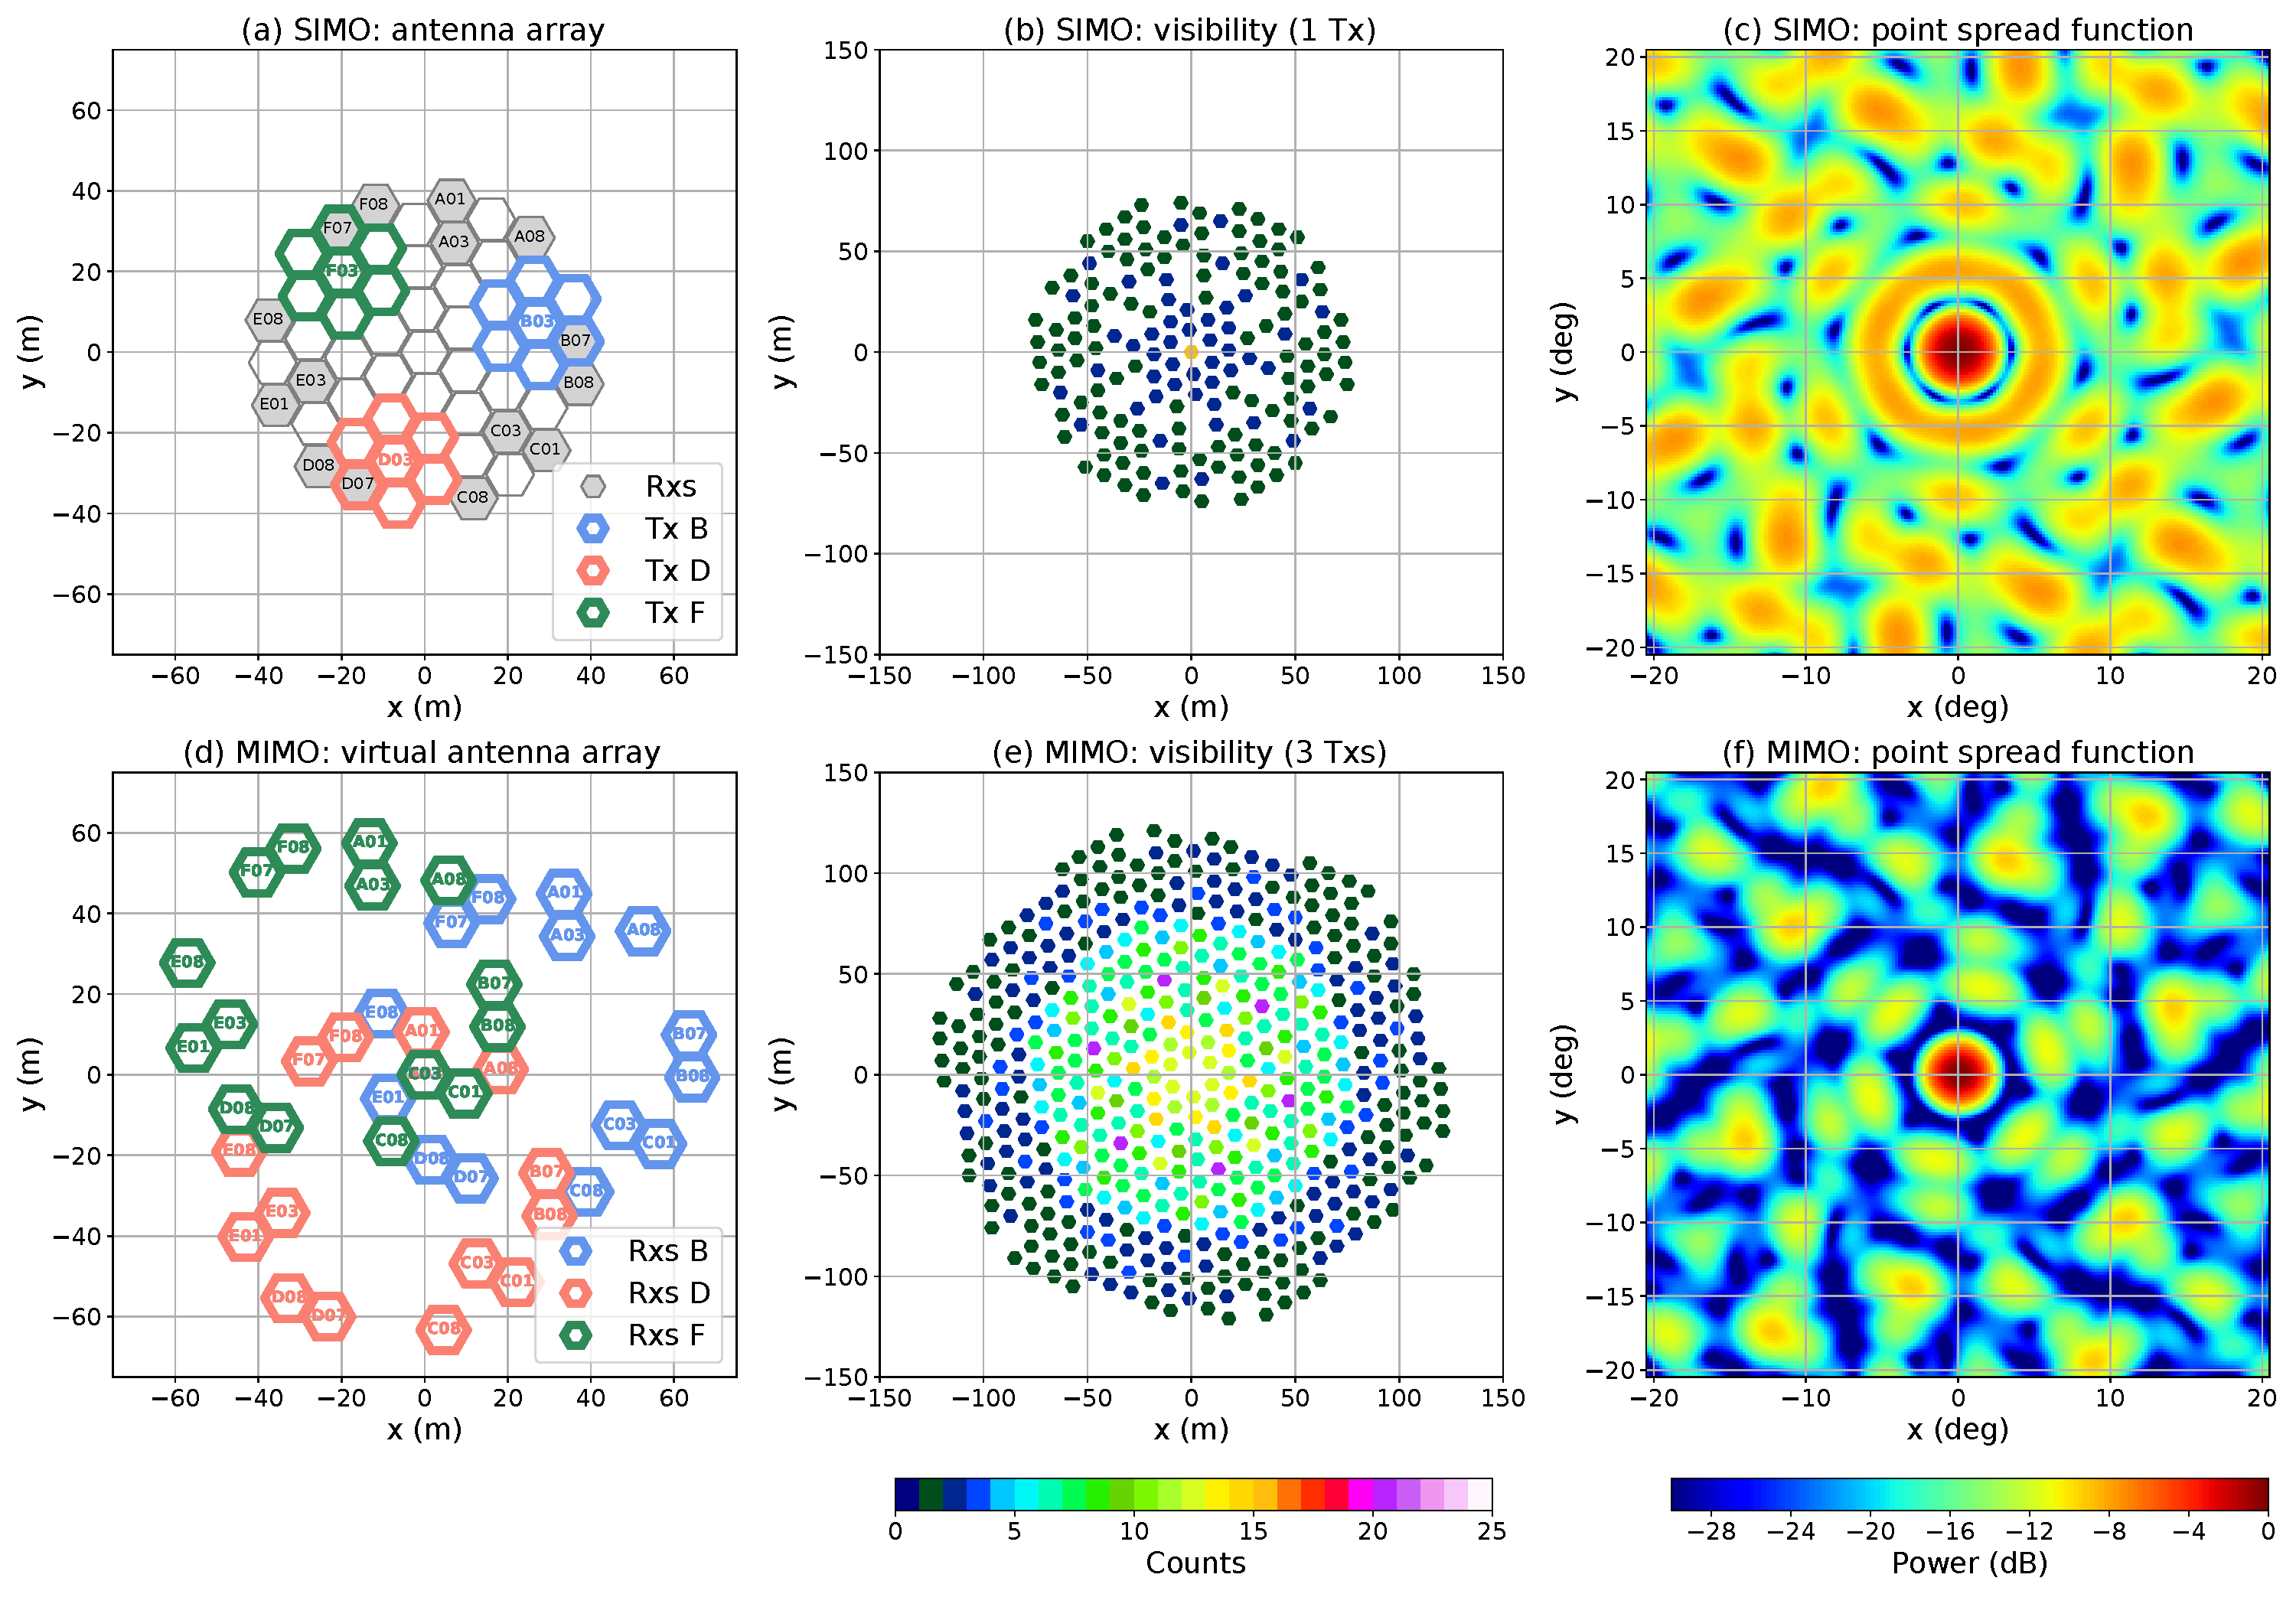
\includegraphics[width=1\linewidth]{figures/amt-12-955-2019-f01-high-res.pdf}
\end{figure}




\vfill

%% Print some more information at the bottom
\begin{tabular}{ll}
    Instructor: & Prof. Gamal Abd El-Fadeil\\
    &Prof. Ahmed Abd El-Halem\\
    Teaching Assistant: & Eng. Basma Diaa \\
    Project Duration: & February , 2026 - Month, 2026 \\
    Faculty: & Faculty of Engineering, Capital University
\end{tabular}

\bigskip
\bigskip


\end{center}

% تأكد من إضافة \usepackage[export]{adjustbox} في مقدمة الملف لدعم valign
\begin{tikzpicture}[remember picture, overlay]
	\node[above=10mm] at (current page.south) {%
		
\includegraphics[width=2.5cm, valign=m]{figures/englogo}  
		
\includegraphics[width=3.5cm, valign=m]{figures/unilogo}
	};
\end{tikzpicture}

\end{titlepage}
